\section{Binding Energy}
\subsection{Formulas and Definitions}
\begin{itemize}
    \item Binding Energy: The energy required to keep the nucleus together. The mass of the nucleus is not equal to the sum of its parts. The mass of the individual nucleons is higher than the mass of the nucleus. The difference is the binding energy.
    \begin{equation}
    Zm_p + Nm_n - M_{\text{Nucleus}} = \text{Binding Energy}  \quad ⇒ \quad Zm_p + Nm_n > M_{\text{Nucleus}}
    \end{equation}
\end{itemize}

\subsection{Mass of the Nucleus}
The total mass of the atom is the mass of the nucleus and electrons, minus the binding energy of the electrons. 
\begin{equation}
M_{\text{Atom}} = M_{\text{Nucleus}} + Zm_e - \underbrace{∑_{i=1}^{Z} B_i / c^2}_{\text{Often negligible}}
\end{equation}

\begin{equation}
M_{\text{Atom}} = M_{\text{Nucleus}} + Zm_e
\end{equation}

$M$ usually refers to the mass of the entire atom, and so the subscript "Atom" is often omitted. We usually write the atom using the following notation:
\begin{equation}
M\left(_{Z}^{A}X_{N}\right) = M_{\text{Nucleus}} \left(_{Z}^{A}X_{N}\right) + Zm_e
\end{equation}
Multiplying by $c^2$ we get the mass in energy units ($E = mc^2$):
\begin{equation}
M_{\text{Nucleus}}\left(_{Z}^{A}X_{N}\right) = M\left(_{Z}^{A}X_{N}\right) - Zm_ec^2
\end{equation}
\begin{equation}
\underline{\underline{M_{\text{Nucleus}}\left(_{Z}^{A}X_{N}\right)c^2 = M\left(_{Z}^{A}X_{N}\right)c^2 - Zm_e c^2 
}}
\end{equation}
\subsection{Nuclear Binding Energy (B.E.)}
This energy is very small compared to the mass energy of the nucleus. We can derive this from the mass of the nucleus. 
\begin{align}
    B.E. &= \left(Zm_{p} + Nm_{n} - M_{N}\left(_{Z}^{A}X_{N}\right)\right) c^2 \\
    &= \left(Zm_{p} + Nm_{n} - \left(M\left(_{Z}^{A}X_{N}\right) - Zm_e\right)\right) c^2 \\ 
    &= \left(Z(\underbrace{m_{p} + m_e}_{\text{Hydrogen}}) + Nm_{n} - M\left(_{Z}^{A}X_{N}\right)\right) c^2 \\ \\
   B.E. &= \underline{\underline{\left(Zm\left(^{1}H\right) + Nm_{n} - M\left(_{Z}^{A}X_{N}\right)\right) c^2}}
\end{align}
As the units so far has been energy $(mc^2)$ we can switch to MeV. 
\begin{equation}
B.E. = \left[mc^2\right] = \left[uc^2\right] = u931.5\text{MeV /}u \quad ⇒ \quad c^2 = 931.5 \text{MeV/u}
\end{equation}
\begin{equation}\label{eq: binding_energy}
B.E. = \underline{\underline{\left(Zm\left(^{1}H\right) + Nm_{n} - M\left(_{Z}^{A}X_{N}\right)\right) 931.5 \text{MeV/u}}}
\end{equation}

\subsubsection{Example: Helium \protect{$_{2}^{4}H_{2}$}}
We use the formula for binding energy from \cref{eq: binding_energy} to calculate the binding energy of the hydrogen atom $_{2}^{4}He_{2}$.
\begin{align}
B.E. &= \left(2m_p + 2m_n - M\left(_{2}^{4}He_{2}\right)\right) 931.5 \text{MeV/u} \\
&= \left(2 ⋅ 1.007825u + 2 ⋅ 1.008664u - 4.002603u\right) ⋅ 931.5 \text{MeV/u} \\
&= \underline{\underline{0.0304 ⋅  931.5 \text{ MeV} = 28.3 \text{ MeV}}}\label{eq: helium_binding_energy}
\end{align}
The ratio between the binding energy and the rest mass of the nucleus is very small. Using the binding energy from \cref{eq: helium_binding_energy} and the mass of the helium nucleus, we can calculate the ratio:
\begin{equation}
\frac{28.3}{3728} = 0.75\%
\end{equation}
\subsection{Nuclear Separation Energy}
The energy required to separate a proton $S_{p}$ or a neutron $S_{n}$ from the nucleus.
\subsubsection{Neutron Separation Energy}\label{sssec: neutron_separation_energy}
It requires lower energy to remove a neutron from a nucleus with an odd number of neutrons. This is because one is unpaired. 
\begin{equation}
S_n = \left(M\left(_{Z}^{A-1}X_{N-1}\right) - M(_{Z}^{A}X_{N} + m_n)\right)c^2
\end{equation}
This can also be expressed using binding energies as mass and energy are equivalent through $E = mc^2$:
\begin{equation}
S_n = B\left(_{Z}^{A}X_{N}\right) - B\left(_{Z}^{A-1}X_{N-1}\right)
\end{equation}

\subsubsection{Proton Separation Energy}
Using the same logic as for the neutron separation energy \cref{sssec: neutron_separation_energy}, we can express the proton separation energy through the binding energies. It's important to keep in mind that after loosing a proton, the element changes.
\begin{equation}
S_p= \left(M\left(_{Z-1}^{A-1}Y_{N}\right) - M(_{Z}^{A}X_{N} + \underbrace{m_p + m_n}_{_{1}^{1}H_{}})\right)c^2
\end{equation}
\begin{equation}
S_p = B\left(_{Z}^{A}X_{N}\right) - B\left(_{Z-1}^{A-1}Y_{N}\right)
\end{equation}

\subsection{Average Binding Energy}
\begin{itemize}
    \item Except for very light nuclei, the binding energy per nucleon is linear. It's almost constant at around 8 MeV/nucleon.
    \item The highest binding energy per nucleon is around $A = 60$ with the highest binding energy per nucleon at $^{56}\text{Fe}$. 
    \item When going from heavier elements towards iron we get nuclear fission
    \item When going from lighter elements towards iron we get nuclear fusion
\end{itemize}

\begin{figure}[h!]
\centering
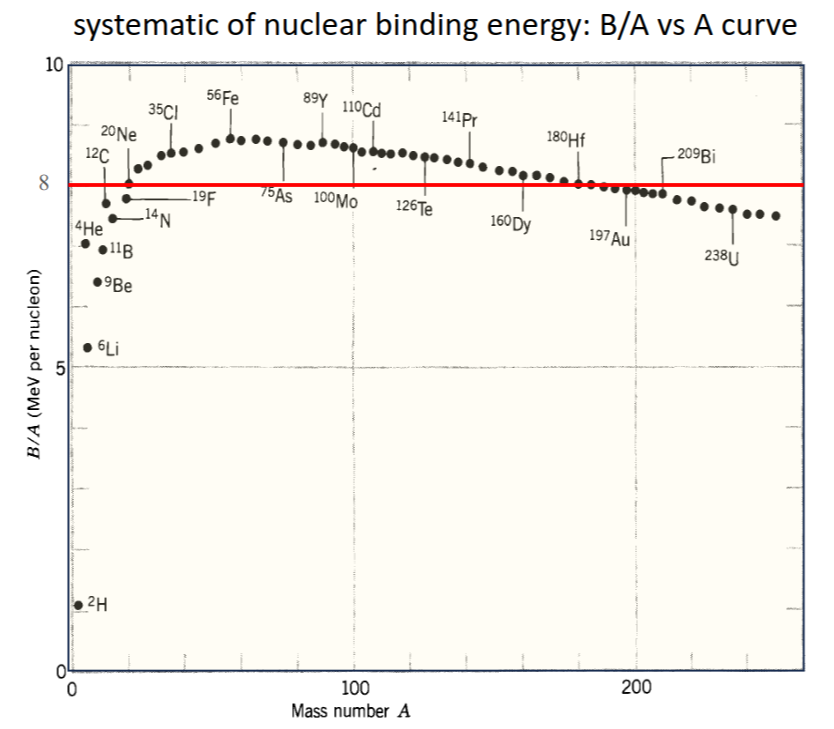
\includegraphics[width = .75\textwidth]{BE_per_nucleon.png}
\caption{}
\label{fig: BE_per_nucleon}
\end{figure}

\subsection{Semi-Empirical Mass Formula}
\begin{itemize}
    \item Sets out to explain the binding energies of nuclei.
    \item It is semi-empirical as the five of its constant are found by experiment.
    \item Tries to recreate the binding energy per nucleus graph in \cref{fig: BE_per_nucleon} by using the \textit{liquid drop model}.
\end{itemize}

\begin{equation}\label{eq: semi_empirical_mass_formula}
B = a_vA - a_sA^{2 / 3} - a_c\frac{Z(Z-1)}{A^{1 / 3}} - a_{\text{asym}}\frac{(A-2Z)^2}{A} + δ
\end{equation}
\subsubsection{Explanation of the Terms in the Semi-Empirical Mass Formula}\label{sssec: Explenation of the Terms in the Semi-Empirical Mass Formula}
\begin{itemize}
    \item $\mathbf{a_vA}$: \textbf{Volume term}. The binding energy is proportional to the volume of the nucleus approximated to a sphere $\left(V = 4πR^3/3\right)$. This dominates the binding energy for large nuclei. 
    \begin{equation}
    a_v ≈ 15.8 \text{ MeV}
    \end{equation}
    The linear dependence of the binding energy on the number of nucleons tells us that the strong force is short range as each nucleon only interacts with its nearest neighbors. 
    \item $\mathbf{a_sA^{2 / 3}}$: \textbf{Surface term}. The volume term is not quite accurate as the nucleons on the surface have fewer neighbors. This term corrects for that. The binding energy is proportional to $πR^2$
    \begin{equation}
    a_s ≈ 16.8 \text{ MeV}
    \end{equation} 
    \item $\mathbf{a_cZ(Z-1)A^{-1 / 3}}$: \textbf{Coulomb term}. The binding energy is reduced by the repulsion between the protons. It is therefore detracted. The Coulomb force is long range and is therefore proportional to $Z(Z-1)$ as all protons interact. 
    \begin{equation}
    a_c ≈ 0.72 \text{ MeV}
    \end{equation}
    \item $\mathbf{a_{\text{asym}}(A-2Z)^2A^{-1}}$: \textbf{Asymmetry term}. Stable nuclei have a balance between protons and neutrons. As the ratio of protons to neutrons deviate from 1, the nuclei becomes less stable (lower binding energy). This inhibits Hydrogen or Helium atoms with many neutrons. It is caused by the Pauli exclusion principle as nucleons are fermions and therefore can not occupy the same state at once. 
    \begin{equation}
    a_{\text{asym}} ≈ 23 \text{ MeV}
    \end{equation}
    Heavier nuclei must have more neutrons to fight the Coulomb repulsion. The term gets relatively small as the number of nucleons increases. 
    \item $\mathbf{δ}$: \textbf{Pairing term}. This term is not included in the original formula, but is added to account for the fact that nuclei with an even number of protons and neutrons are more stable. This is because the nucleons in the same space-state can be coupled to have a total spin of 0. They are therefore closer together and therefore more tightly bound with a higher binding energy. This is called even-even nuclei. 
    \begin{equation}
    δ =  \begin{cases}
        +a_pS^{-3 / 4}, &\text{ if even(N)-even(Z)}\\
        0, &\text{ if odd(A)}\\
        -a_pS^{-3 / 4}, &\text{ if odd(N)-odd(Z)}\\
    \end{cases} 
    \end{equation}
    \begin{equation}
    a_p ≈ 34 \text{ MeV}
    \end{equation}
\end{itemize}
\subsubsection{SEMF Conclusion}
\begin{itemize}
    \item The semi-empirical mass formula was a first attempt at understanding how binding energy works. 
    \item It is semi-empirical as the constants are found by experiment. 
    \item A negative binding energy means the nucleus is not bound and is therefore not stable.
\end{itemize}
\begin{equation}
B = \underbrace{a_vA - a_sA^{2 / 3} - a_cZ(Z-1)A^{-1 / 3}}_{\text{Liquid-drop model for energy calculations}} - \underbrace{a_{\text{asym}}(A-2Z)^2A^{-1} + δ}_{\text{Interactions between nucleons}}
\end{equation}
\begin{figure}[h!]
\centering
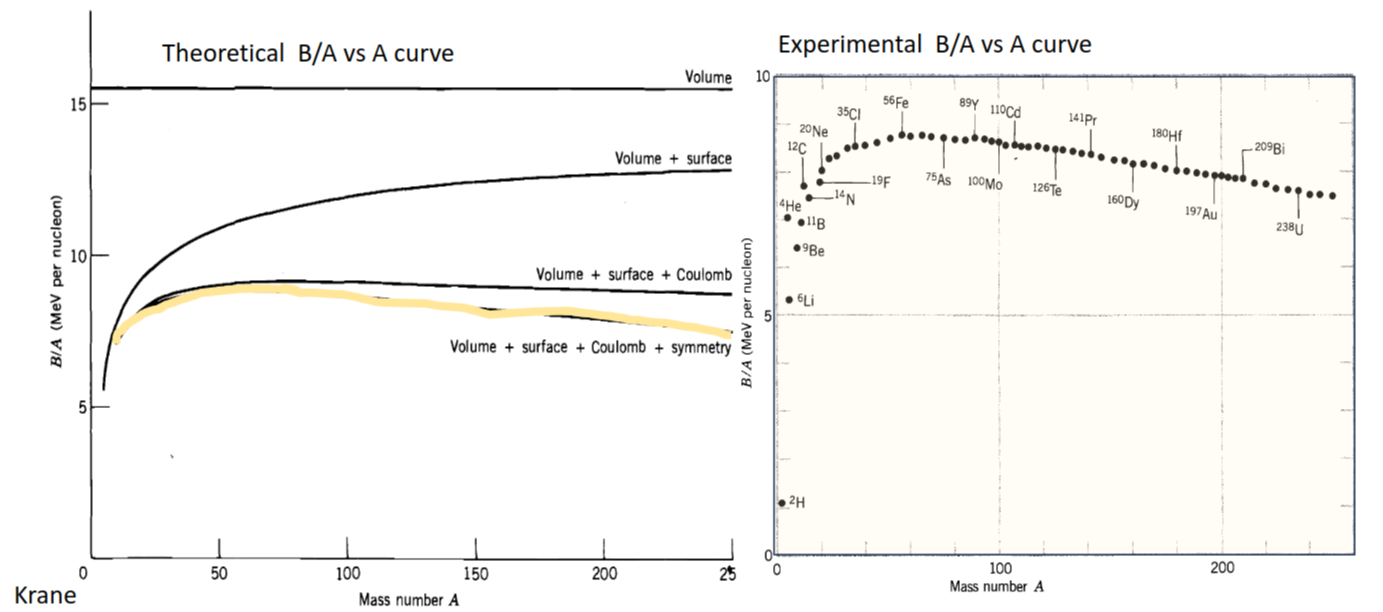
\includegraphics[width = \textwidth]{SEMF_term_addition.png}
\caption{Plot of how the different terms in the semi-empirical mass formula \cref{eq: semi_empirical_mass_formula} gets us closer to the experimental values}
\label{fig: SEMF_term_addition}
\end{figure}



